\subsection{\ga with Guided Local Search}
\label{sec:GALS}

Purely random mutation requires many generations to converge. To enhance the exploration performance, \ga employs a guided local search inspired by ~\cite{wen2011heuristic}. For each chromosome it searches for the best neighbor to propagate (instead of random mutation). The evaluation methodology for the local search is crucial for the overall exploration performance. \ga uses a hybrid approach between Domain Score (DS) and Analytic Evaluation (AE) model. In order to simplify explanation and to enable details analysis, we introduce two simpler variants first: \gads and \gaana.

%It first finds the best neighbor of a chromosome by exhaustively switching two genes with opposite states (i.e. replacing a function type for HW implementation), and then evaluates the benefit of each swap. With respect to evaluation method, we proposed three variations: (1) \gads, (2) \gaana, and (3) \gah which is the ultimate \ga implementation. 

%Instead of the random mutation implemented in GA-Random,  \emph{\gads} performs a guided local search, see \figref{fig:GADSS}, 

%We consider three variants (sorted by complexity) for guided local search: (1) a guided local search using the proposed Domain Score (\gads), (2) a guided local search using the proposed Analytical Model (\gaana) for evaluation, (3) our complete approach, \ga, which employs a hybrid DS and Analytical Model, combining their benefits.  


\subsubsection{\gads}
\label{sec:GALS-DSS}

\figref{fig:GADSS} illustrates the guided local search used instead of random mutation of \garand. \gads finds the best neighbor of a chromosome $Ch_{cur}$ by exhaustively switching two genes with opposite states, and then evaluates the benefit of each swap using \newtext{the Domain Score (DS),} see~\secref{sec:ds}.

\newtext{After finding the best neighbor}, \gads keeps the best neighbor $Ch_{BN}$ (i.e. mutation with the most benefit) over the starting chromosome $Ch_{cur}$. If the best neighbor $Ch_{BN}$ improves DS, it then becomes $Ch_{cur}$ the starting point for the next search and the process repeats. 

The search terminates if no improvement is found. The last $Ch_{BN}$ becomes one chromosome in next generation. If the first search iteration does not find any improvement, the search terminates immediately and instead of $Ch_{cur}$ a new random chromosome $Ch_{R}$ is inserted. This increases the random variation and thus the chance to escape a local optimum in the following generation(s). The local search process repeats for each chromosome $Ch0' .. Chn'$. 



\begin{figure}[h]
	\centering
	%\vspace{-10pt}
	\subfloat[GA-LS(DS),GA-LS(AE) ]{
		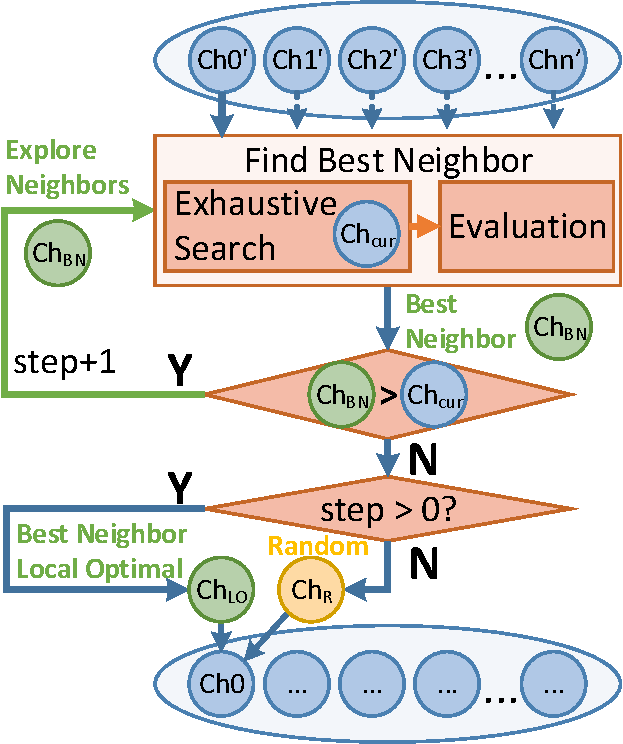
\includegraphics[width=.45\linewidth]{fig/pGADSS.pdf}
		\label{fig:GADSS}}
	\hfill
	\subfloat[GA-LS(Hybrid)]{
		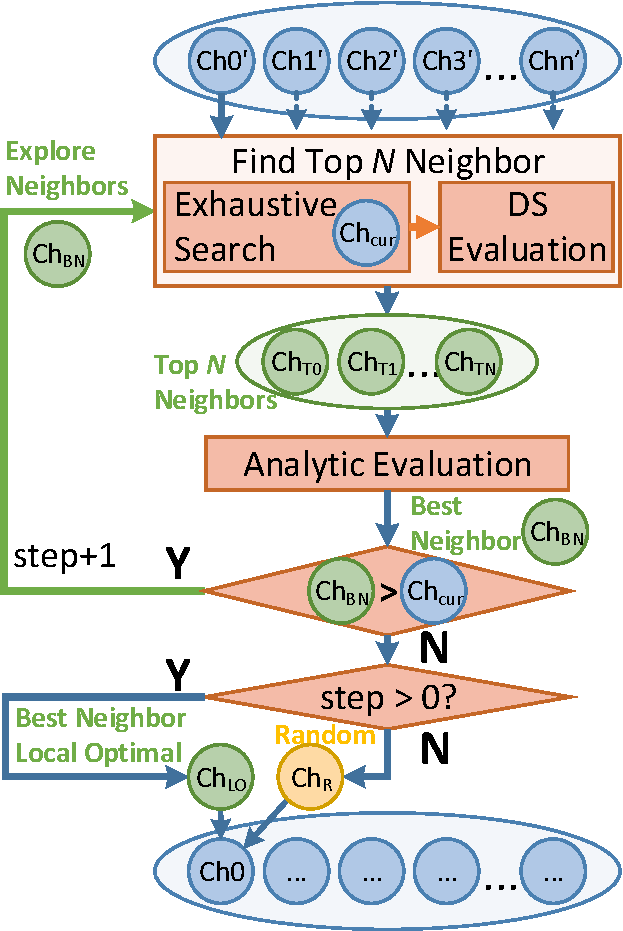
\includegraphics[width=.45\linewidth]{fig/pGADSSA.pdf}
		\label{fig:GAHybrid}}
	%\vspace{-5pt}
	\caption{Guided Local Search}
	%\vspace{-8pt}
\end{figure}

%Local search an iterative algorithm that starts with one solution, then attempts to find the best neighbor solution by exhaustive evaluate all neighbors. If the best neighbor produces a better solution compared with the original one, the best neighbor is made to the new solution, repeating until no further improvements can be found.
%In our GA algorithm, the solution is the chromosome, which defining the domain SW / HW partitioning. The neighbors of the chromosome, are (1) migrating one function type from SW(HW) to HW(SW), and (2) swap a pair of function types between SW and HW.

%Apply local search for each chromosome in generation. Using DSS to evaluate all neighbors of this chromosome, and find the best neighbors as the next step, if it has improvement. Search until no longer improvement. At the end, the mutation finds top 1 candidate (local optimal architecture) for each chromosome to form the new generation.

%If the original chromosome has been evaluated before or it is already the local optimal solution, which local search step is equal to 0, and cannot find a better neighbor in the first step of local search.
%The GA random generated a new chromosome for next generation, to help our GA to explore the large design space with more diversity.

%TODO GS Idea if the best chromosome was created just by cross over. Then, we will discard it with the approach above and replace it with a random chromosome. In effect: the absolute best solution can only be found through mutation in our setting. Improvement: after selection & chross over to a ranking by DS. Top X% of ranked chromosomes are not displaced by random, if no further improvement is found. 





\subsubsection{\gaana}

The just introduced \emph{\gads} favors speed over accuracy using the DS for evaluation in the neighborhood search. While DS is the fastest evaluation, it has limited accuracy (see \secref{sec:eva:sum}). In order to quantify the impact, we introduce the more accurate \emph{\gaana}. It realizes the same search as \emph{\gads}, however, uses the analytical model for evaluation. As the analytical model computes the performance of a single application, each application in the domain has to be evaluated and the results aggregated to determine the chromosome's fitness. This is identical to the \emph{evaluation} in \emph{\garand}. In result, the \gaana performs a very accurate local search, at the cost of exploration speed. 
\subsubsection{\gah}

In order to combine the benefits of \gads speed  and \gaana accuracy in the local search, we introduce \gah combining both approaches.

The exhaustive search over the local neighbors significantly impacts overall exploration performance. It evaluates many alternatives ($ \sum_{1 .. \lvert P \rvert} Steps_{i} * N * (\lvert T \rvert - N)$). Even considering only 1 step for each chromosome ($\lvert T \rvert$ = 50, $N$=10), already 5600 alternatives are evaluated. Hence, the fastest evaluation possible is paramount. To achieve this, \gah employs a two step approach: it first uses the faster (but less accurate) DS to identify a group of best neighbor candidates, and then re-evaluates those using the more accurate (but slower) Analytical Model to find the best neighbor. See \figref{fig:GAHybrid}. 

\gah first uses the faster evaluation \emph{DS} to find through exhaustive search the $N$ best neighbors ($Ch_{BN0}$ .. $Ch_{BNN}$) for a given chromosome $Ch_{cur}$. It then uses the analytic evaluation to select the best neighbor $Ch_{BN}$ from these candidates. The termination and random chromosome insertion are identical to \gads.

Dimensioning the group size is a local speed/accuracy trade-off. For our experiments, we opt to compare the top 5 neighbor candidates. We postulate that DS is sufficiently accurate to delineate from 400 down to 5 candidates ($\lvert T \rvert$ = 50, $N$=10). In addition, finding the absolute best in each step is not necessary as the search is iterative, improving in the next local step (or generation).


%\begin{figure}[htbp]
%	\centering
%	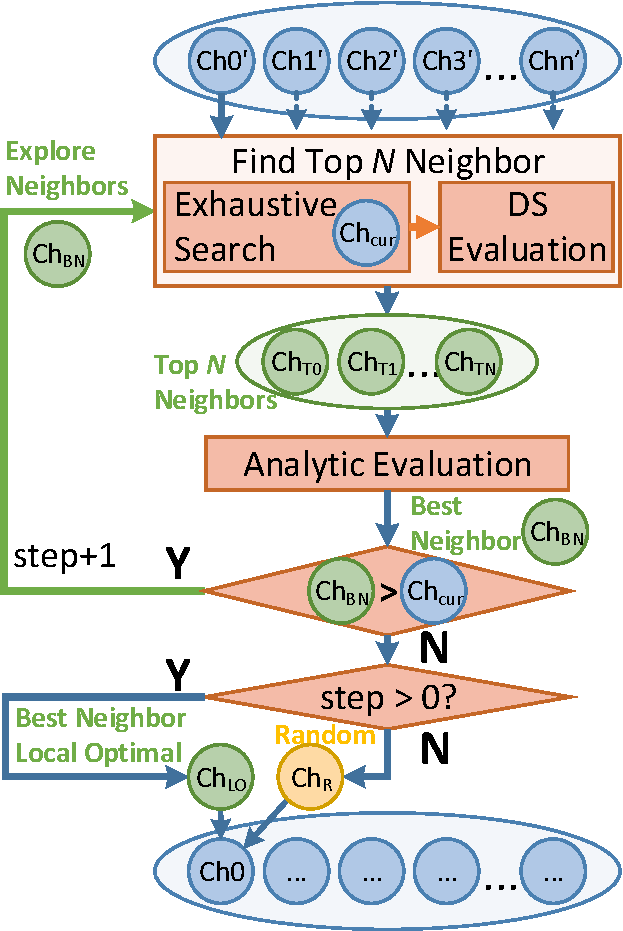
\includegraphics[width=0.48\linewidth]{fig/pGADSSA.pdf}
%	\caption{Guided Local Search (Hybrid)}
%	\label{fig:GAHybrid}
%\end{figure}
